% Multiple Choice Question 7

\begin{center}
    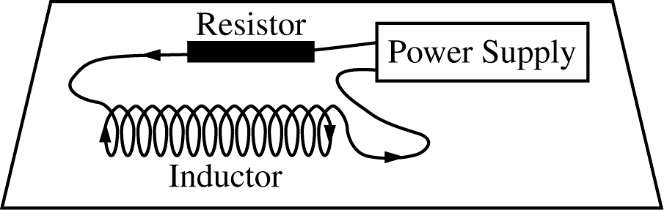
\includegraphics[scale=0.3]{images/img-005-009.png}
\end{center}

\begin{questions}
\setcounter{question}{6}

\question
An inductor with inductance $L=0.30 \unit{H}$ is connected in series with a resistor and both are connected to a power supply, as shown above. The power supply generates a current $I$ that is given as a function of time $t$ by the equation $I=I_{0}(1-t/k)$, where $I_{0}=4.0 \unit{A}$ and $k=2.0 \unit{s}$. What is the magnitude of the potential difference across the inductor induced by the changing current?

\begin{oneparchoices}
    \choice $0.15 \unit{V}$
    \choice $0.30 \unit{V}$
    \choice $0.60 \unit{V}$
    \choice $1.2 \unit{V}$
    \choice $2.4 \unit{V}$
\end{oneparchoices}

\end{questions}
